\section{System overview}

This report provides information on an all-digital FM stereo modulator developed as a final project for Projecto de Sistemas Digitais. 

A general overview of the project and its sub-modules can be seen in \autoref{fig:overview}.

\begin{figure}[!h]
\centering
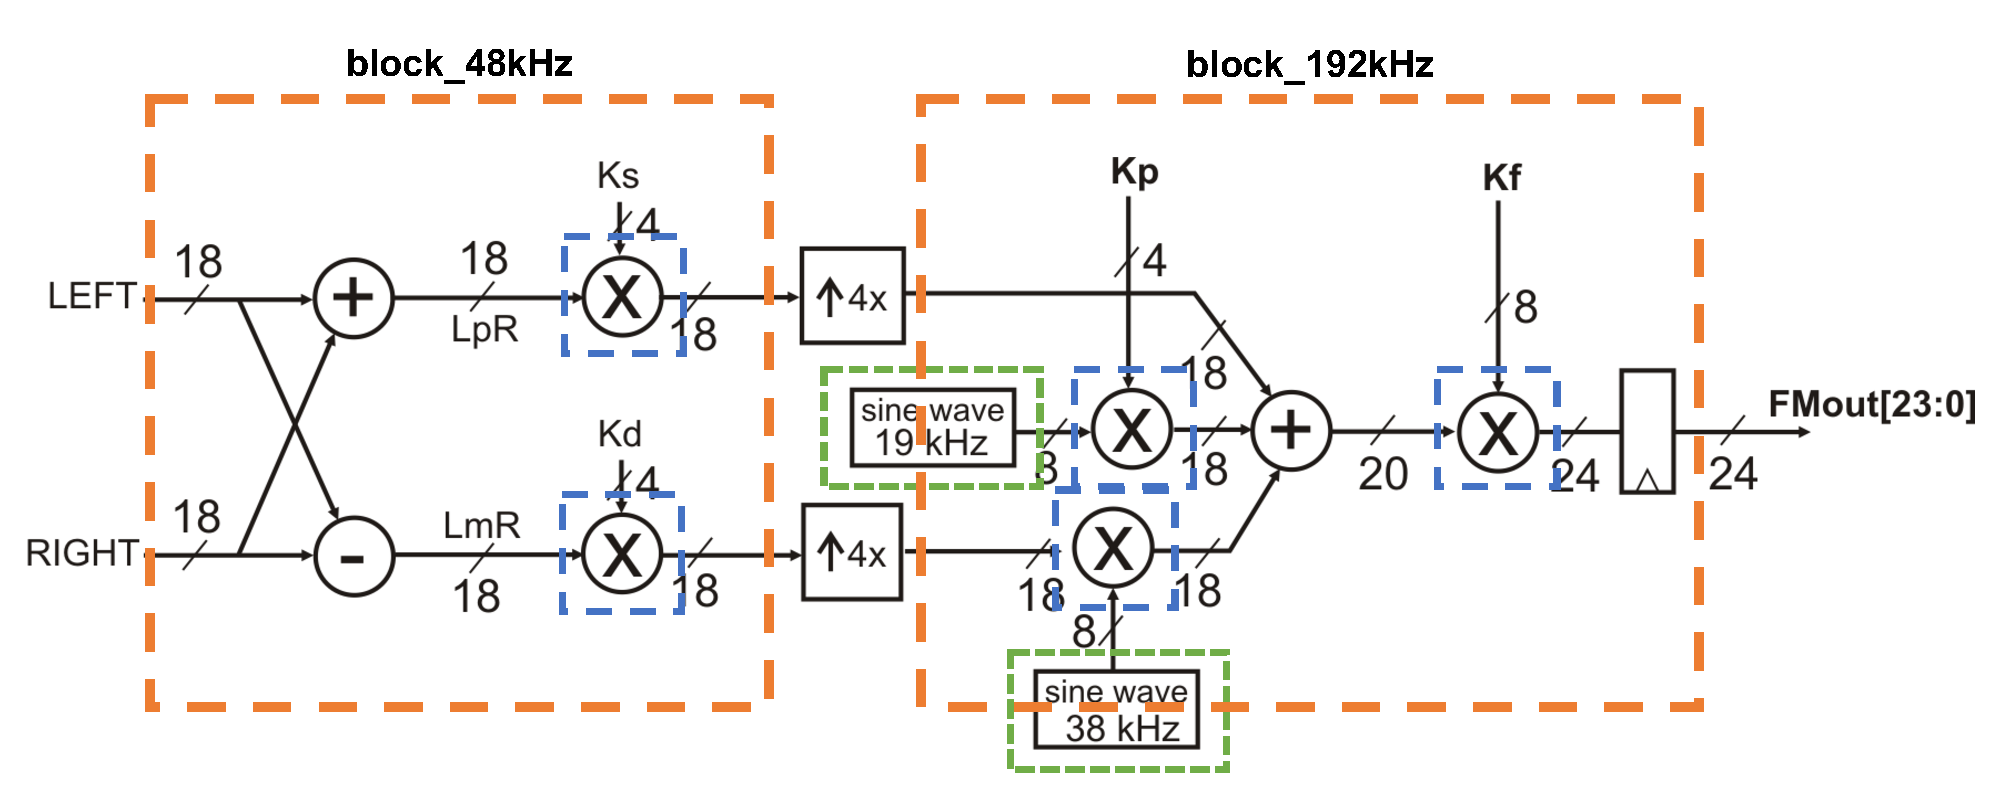
\includegraphics[width=0.7\textwidth,height=0.2\textheight]{overview.pdf}
\caption{Block diagram overview of the project. Implemented macro blocks are highlighted in orange; DDS blocks are seen in green; improved multiplication blocks are seen in blue.}\label{fig:overview}
\end{figure}

The implementation of this project was wrapped under a single module named \texttt{my\_fm\_module}, which was split into the following blocks:

\begin{itemize}
	\item \texttt{block\_48kHz}: corresponds to the leftmost block, which receives the stereo input at a sample rate of 48 kHz. Its outputs will feed each of the interpolators.
	\item \texttt{interpol\_4x}: interpolate the signal for further processing. The blocks used were provided as IP blocks.
	\item \texttt{block\_192kHz}: corresponds to the rightmost block, which processes the signal at a rate of 192 kHz. It outputs the final FM signal.
\end{itemize}

Besides this, two additional modules were implemented:
\begin{itemize}
	\item \texttt{dds}: implements each of the sine wave generators. Implementation details can be read in \autoref{sec:dds-module}.
	\item \texttt{seqmultNM\_sat}: implements a wrapper of the original \texttt{seqmultNM} IP block. It implements some of the control logic detailed in \autoref{sec:control-path}, as well as a comprehensive mechanism that allows for rescaling the number and for saturating the output, thus avoiding overflow.
\end{itemize}

All sums and shifting operations were performed using standard Verilog code.

Furthermore, some optimisations were performed throughout the implementation of the project. These are described under \autoref{sec:further-optimisations}.
